\chapter{Results}\label{ch:results}

\section{Predicted and Observed Event Yields}\label{sec:results_yields}

Figure~\ref{fig:results_mj_dists} shows the predicted and observed $M_J^{\Sigma}$ distributions in the
four-jet and five-jet regions, along with the total estimated background uncertainty.

The red solid line indicates the estimated yield in each $M_J^{\Sigma}$ bin, and the red shaded area
shows the total uncertainty, including statistical and systematic uncertainties.

The gray dashed lines are the $\pm1\sigma$ bands from the statistical uncertaity only.

There is good agreement between predicted and observed event yields across a range of $\pm1\sigma$ values,
within the total uncertainty.

The exception is in the five-jet signal region, where a slight excess of events is observed.

After statistical analysis, discussed in~\ref{sec:results_stats}, the excess is found to not be significant.

The $M_J^{\Sigma}$ distributions for two different cascade decay signal mass points are also shown on the plots,
to visualize the effect that the existence of signal events would hve on the distributions.


\begin{figure}[!ht]
    \centering
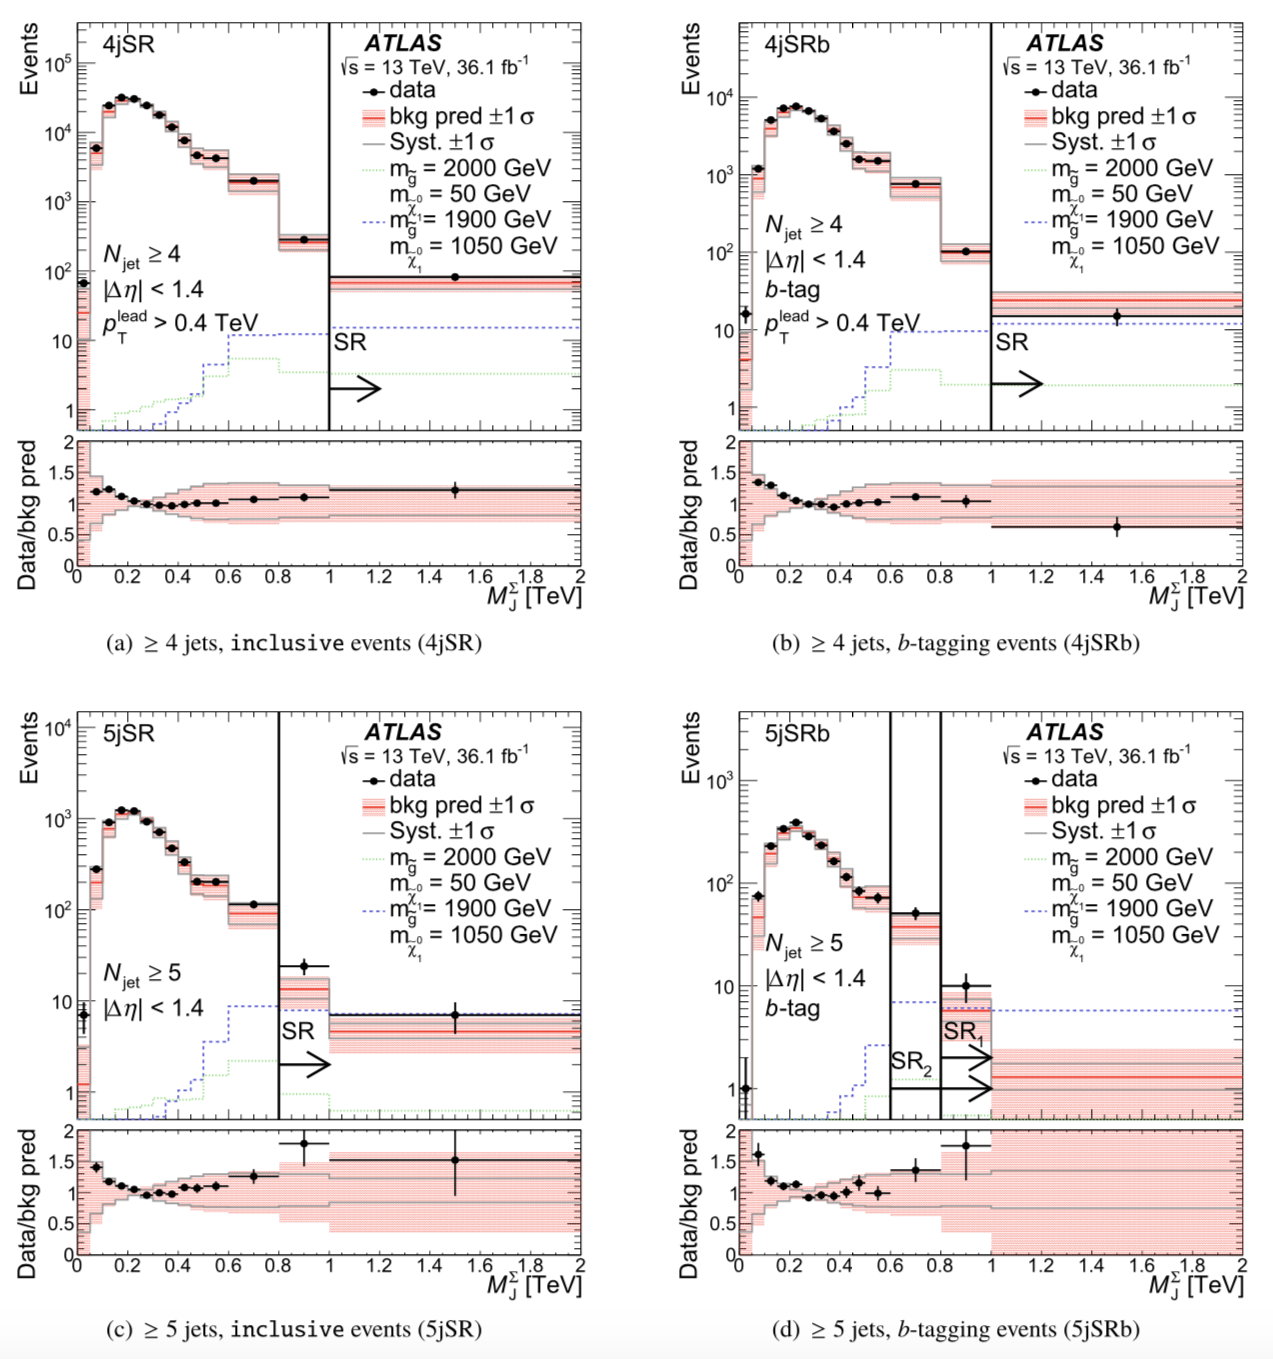
\includegraphics[width=0.8\linewidth]{results_mj_dists}
\caption{Distribution of $M_J^{\Sigma}$ in the four-jet inclusive (4jSR), four-jet b-tag (4jSRb), five-jet inclusive
(5jSR), and five-jet b-tag (5jSRb) regions.
The solid red lines show the predicted $M_J^{\Sigma}$ distributions, along with the total uncertainty shaded in red.
The black dots show the observed $M_J^{\Sigma}$ distributions.
The corresponding $M_J^{\Sigma}$ cuts are indicated with the solid black vertical line and arrow for each region.
Two separate signal regions are defined for the 5jSRb region, one with an $M_J^{\Sigma}$ cut of $0.6~TeV$,
and one with a cut of $0.8~TeV$.
The green and blue dashed lines show the predicted $M_J^{\Sigma}$ contribution from cascade-decay signal events
from two different mass points.
}
\label{fig:results_mj_dists}
\end{figure}

In the four-jet signal regions, no excess of events was observed.
In the five-jet signal regions, an excess of events were observed, but these excesses are not statistically
significant.

Predicted and observed yields in all signal regions are shown in table~\ref{tbl:results_yields_table},
including the number of events in the corresponding normalization region, $N_{NR}$, and the statistical and systematic
uncertainties on the background yield predictions in those regions.

Table~\ref{tbl:results_yields_table} also shows the number of events in the normalization region, $N_{NR}$,
corresponding to each signal region.

The central value of the prediction for each signal region is shown, as well as the statistical uncertainty,
and the systematic uncertainties from the low-$p_T$ and high-$p_T$ uncertainty determination regions.

\begin{table}[!ht]
    \centering
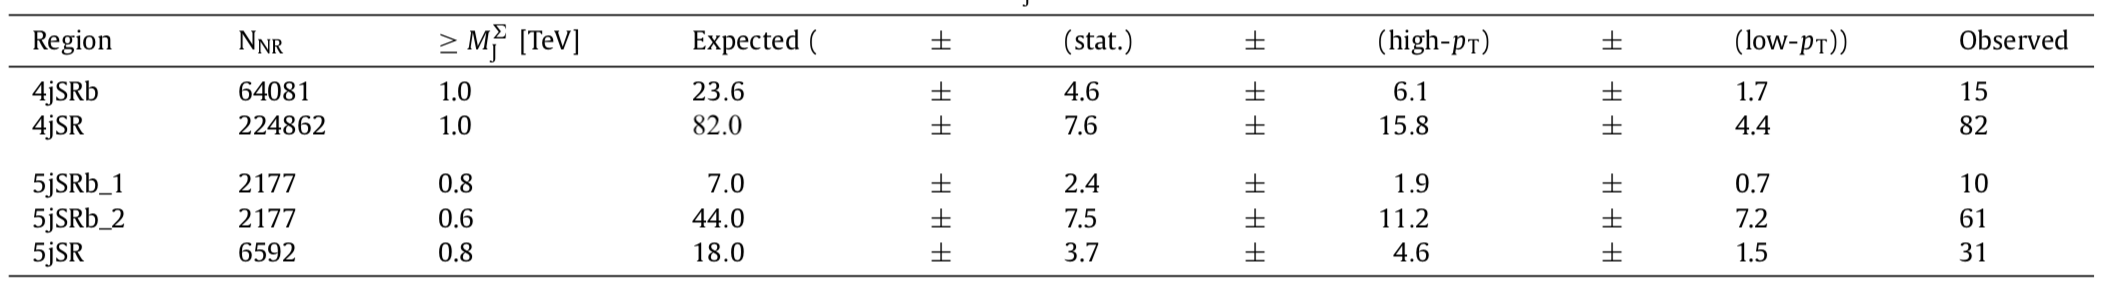
\includegraphics[width=0.8\linewidth]{results_yields_table}
\caption{Predicted and observed yields in all signal regions used in the analysis.
The number of events in the corresponding normalization regions, $N_{NR}$ is shown.
For each signal region, the minimum value of $M_J^{\Sigma}$ used to define that region is also shown.
Additionally, the statistical uncertainty on the background yield, as well as the two systematic uncertainties,
derived from the high-$p_T$ and low-$p_T$ UDRs are shown~\cite{paper-plb}.}
\label{tbl:results_yields_table}
\end{table}

\section{Statistical Interpretation}\label{sec:results_stats}

\subsection{Determining the significance of an excess over the background prediction}\label{subsec:results_stats_excess}
In order to determine if the excesses seen in the five-jet signal regions are statistically significant,
a hypothesis test was conducted, using the likelihood ratio method~\cite{results-stats-asymptotic}.

In this case, the null hypothesis, $H_0$ is the hypothesis that the signal process does not exist, and that the
background prediction is true.

The p-value will therefore quantify the probability of observing an event yield at least as large as that observed,
under the assumption that the signal process does not exist.

Statistical uncertainties on the signal and background yields are incorporated as nuisance parameters in the likelihood
function.

The resulting p-values for the signal regions can be seen in table~\ref{tbl:results_model_ind_limits}.
No signal region shows a statistically significant deviation from the background prediction.

\begin{table}[!ht]
    \centering
    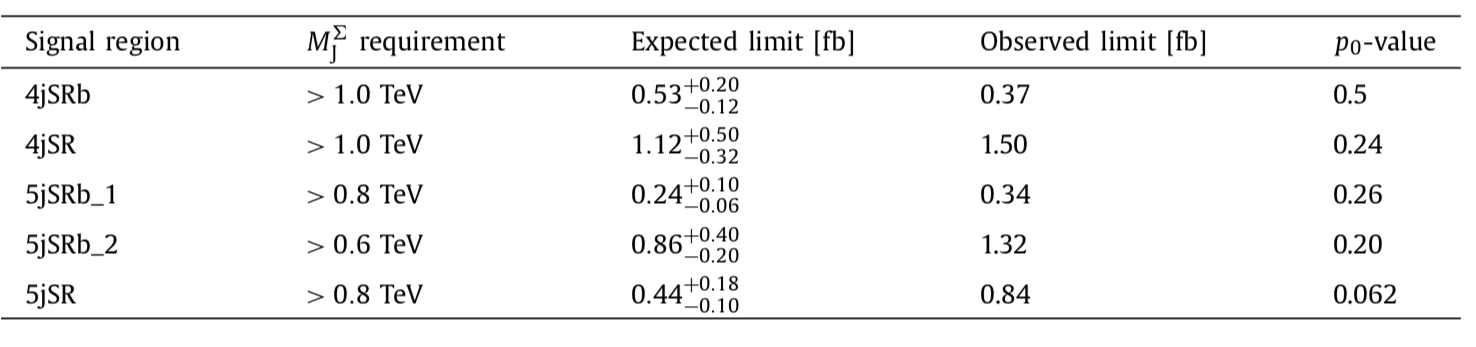
\includegraphics[width=0.8\linewidth]{results_model_ind_limits}
    \caption{Observed and expected limits on gluino pair-production cross section for each of the signal regions,
    along with the p-value for any excess observed in each region~\cite{paper-plb}.}
\label{tbl:results_model_ind_limits}
\end{table}

\subsection{Observed and Expected Limits}\label{subsec:results_limits}

As there was no significant excess of events over the background prediction, no evidence for the signal model was found.
Using the observed yields, upper bounds can be set on the cross-section of the two different
models, as well as model-independent upper bounds.

The limits are determined using the $CL_s$ method, which uses a likelihood ratio test statistic~\cite{results-stats-cls}.

The resulting limits are shown in figure~\ref{fig:results_six_quark_limits}.
The theoretical $\tilde{g}\tilde{g}$ production cross-section as a function of $m_{\tilde{g}}$ is shown as a red dashed
line, with gray band indicating the uncertainty.

The expected limit is shown as a black dashed line with green and yellow bands indicating the one- and two-sigma uncertainty extent.
The observed limit is a solid black line.
Because of the small excess of events observed in the signal region, the upper bound on the production cross section
is higher than the theoretical production cross section in the entire gluino mass range that was tested,
from $900~GeV$ to $1.8~TeV$.

\begin{figure}[!ht]
    \centering
    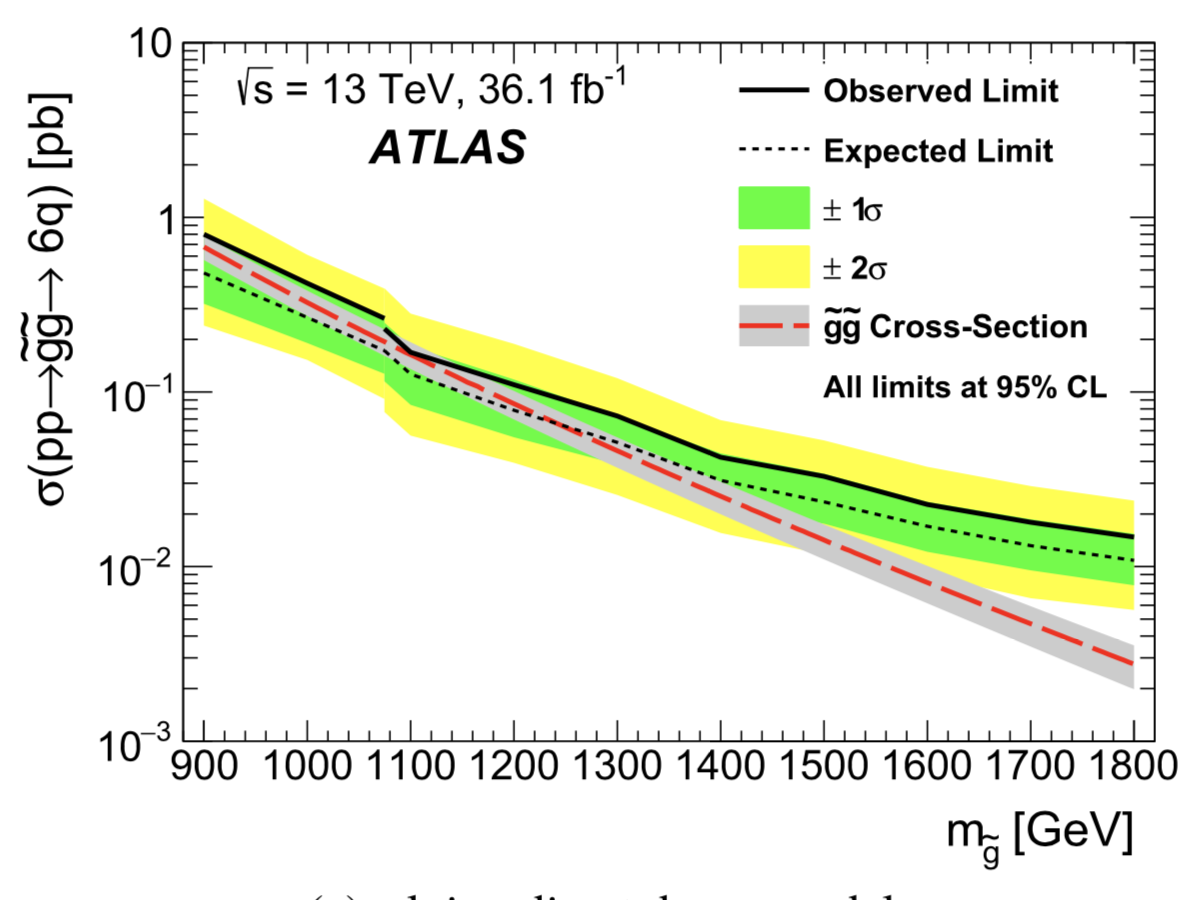
\includegraphics[width=0.8\linewidth]{results_six_quark_limits}
    \caption{Predicted and observed cross-section limits for the direct decay model over a range of $m_{\tilde{g}}$ values.
    Also shown are the estimated gluino pair production cross-sections at each mass point~\cite{paper-plb}.}
\label{fig:results_six_quark_limits}
\end{figure}

For the cascade decay model, limits were set over a range of $m_{\tilde{g}}$ values from $800~GeV$ to $2.2~TeV$,
and for $m_{tilde{\chi}_1^0}$ values from $50~GeV$ to $2.2~TeV$, with $m_{\tilde{g}} > m_{tilde{\chi}_1^0}$.
As with the direct decay model, the limits are worsened by the small excess in the signal regions.

However, a significant portion of the parameter space has been excluded for this model as compared to the Run-1 analysis.
The gluino mass excluded varies from $1~TeV$ to $1.875~TeV$ depending on the value of $m_{tilde{\chi}_1^0}$.

The observed and expected 95\% CL mass exclusions over the  $m_{\tilde{g}} - m_{tilde{\chi}_1^0}$ plane can be seen in figure~\ref{fig:results_ten_quark_limits}.

The observed limit and its theoretical uncertainty are shown in red, the expcted limit is shown in black with 1 sigma band
shown in yellow.

For comparison, the Run 1 limit is shown in gray.

\begin{figure}[!ht]
    \centering
    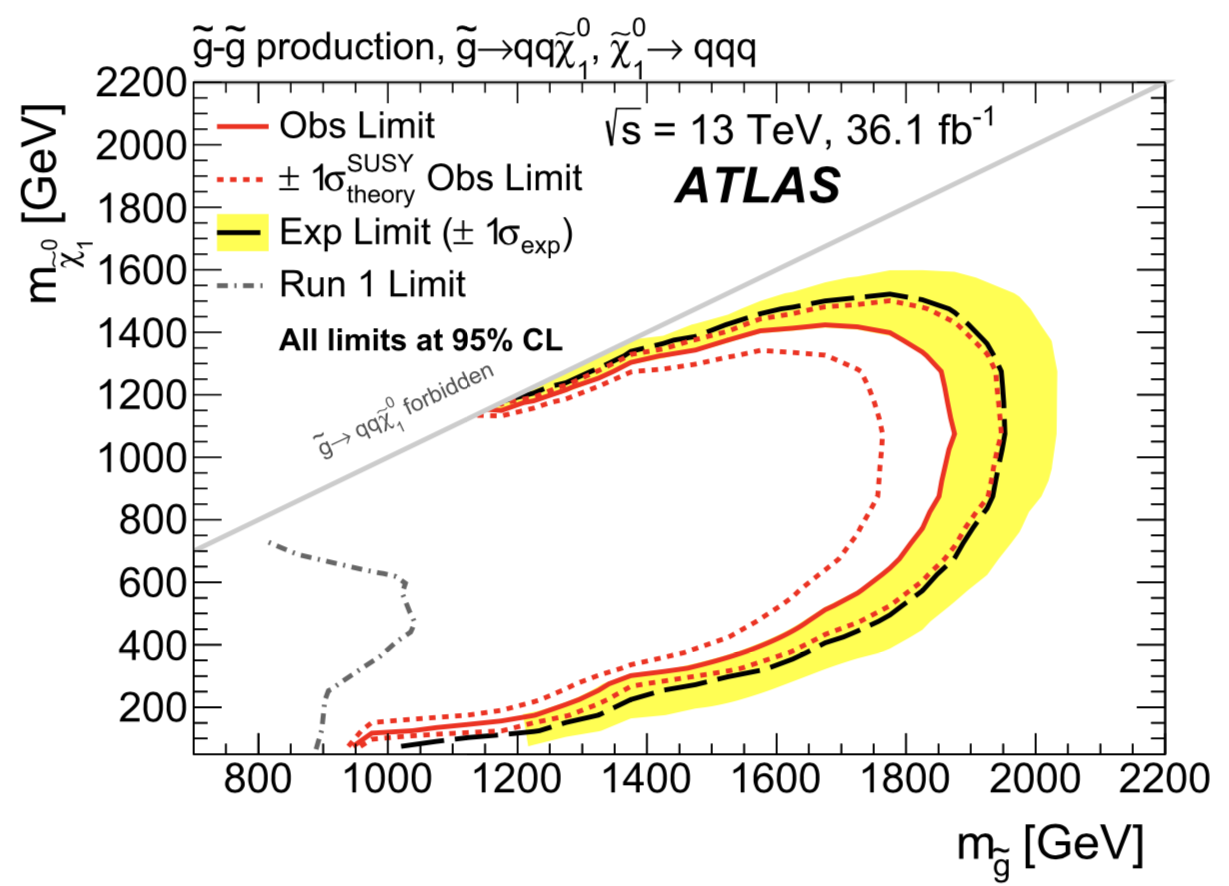
\includegraphics[width=0.8\linewidth]{results_ten_quark_limits}
    \caption{Predicted and observed limits for the cascade decay model over a range of $m_{\tilde{g}}$ and $m_{\tilde{\chi}_1^0}$ values.
    Both predicted and observed limits are shown with $1\sigma$ uncertainty bands.
    The gray dashed curve shows the limits from the Run-1 analysis.
    Due to slight excess in the signal region, the observed limit is less than expected~\cite{paper-plb}.}
\label{fig:results_ten_quark_limits}
\end{figure}

